Il existe  deux techniques pour  r�cup�rer \visidia dot� de  la partie
agents mobiles.  Soit vous  utilisez une version suppos�e stable, soit
vous r�cup�rez une version de d�veloppement. 


\section{R�cup�rer la version stable}

Pour   r�cup�rer    la   version    stable,   allez   sur    le   site
\url{https://developer.berlios.de/projects/visidia/}. Au  milieu de la
page,  vous trouverez  une  section nomm�e  ``Derni�res r�visions  des
fichiers''. Cliquez  alors sur le lien t�l�chargement  et r�cup�rez le
fichier le plus r�cent. Enfin,  d�compressez le fichier � l'aide de la
commande :

\begin{verbatim}
$ tar xvfj lefichiertelecharge.tar.bz2
$
\end{verbatim}


\section{R�cup�rer la version en d�veloppement}

Pour disposer de la version  de d�veloppement, vous devez poss�der SVN
qui   est  un   rempla�ant   de   CVS  disponible   sur   le  site   :
\url{http://subversion.tigris.org/}.\\

Le gestionnaire de version SVN est compil� et disponible sous forme de
paquets pr�s � l'emploi pour la majorit� des distributions Linux. Sous
Windows,   TortoiseSVN   permet   de   travailler  sous   SVN   depuis
l'explorateur   de   fichiers.  Il   est   disponible   sur  le   site
\url{http://www.tortoisesvn.tigris.org/}.\\


Pour  t�l�charger la  version de  d�veloppement, utilisez  la commande
suivante :

\begin{verbatim}
$ svn checkout svn://svn.berlios.de/visidia/trunk/src visidia
$
\end{verbatim}

Cela va cr�er un r�pertoire \dossier{visidia} dans le dossier courant. 


\section{Compiler et lancer \visidia}

Pour compiler  \visidia, le  kit de d�veloppement  Java 5.0  doit �tre
install� et pr�sent dans votre PATH.  Il est disponible sur le site de
SUN   \url{http://java.sun.com/j2se/1.5.0/download.jsp}.\\   Pour   le
v�rifier :

\begin{verbatim}
$ javac -version
javac 1.5.0
$
\end{verbatim}

Placez-vous  dans  le  r�pertoire  \dossier{visidia} et  ex�cuter  les
commandes suivantes pour compiler puis pour lancer \visidia :

\begin{verbatim}
$ ./compile.sh
$ ./acompile.sh
$ ./visidia.sh
$
\end{verbatim}

La premi�re  ligne compile \visidia  alors que la seconde  compile les
modules  comme les algorithmes,  les agents  etc.  La  troisi�me lance
\visidia. Suivant votre installation,  vous pourriez avoir de nombreux
messages d'avertissements concernant les accents. Ces messages ne sont
pas bloquants, vous pouvez les ignorer.\\

Si tout  c'est bien pass�,  \visidia devrait �tre lanc�.  Vous devriez
voir l'application comme sur la figure \ref{fig:visidia}.

\begin{figure}[ht]
  \centering
  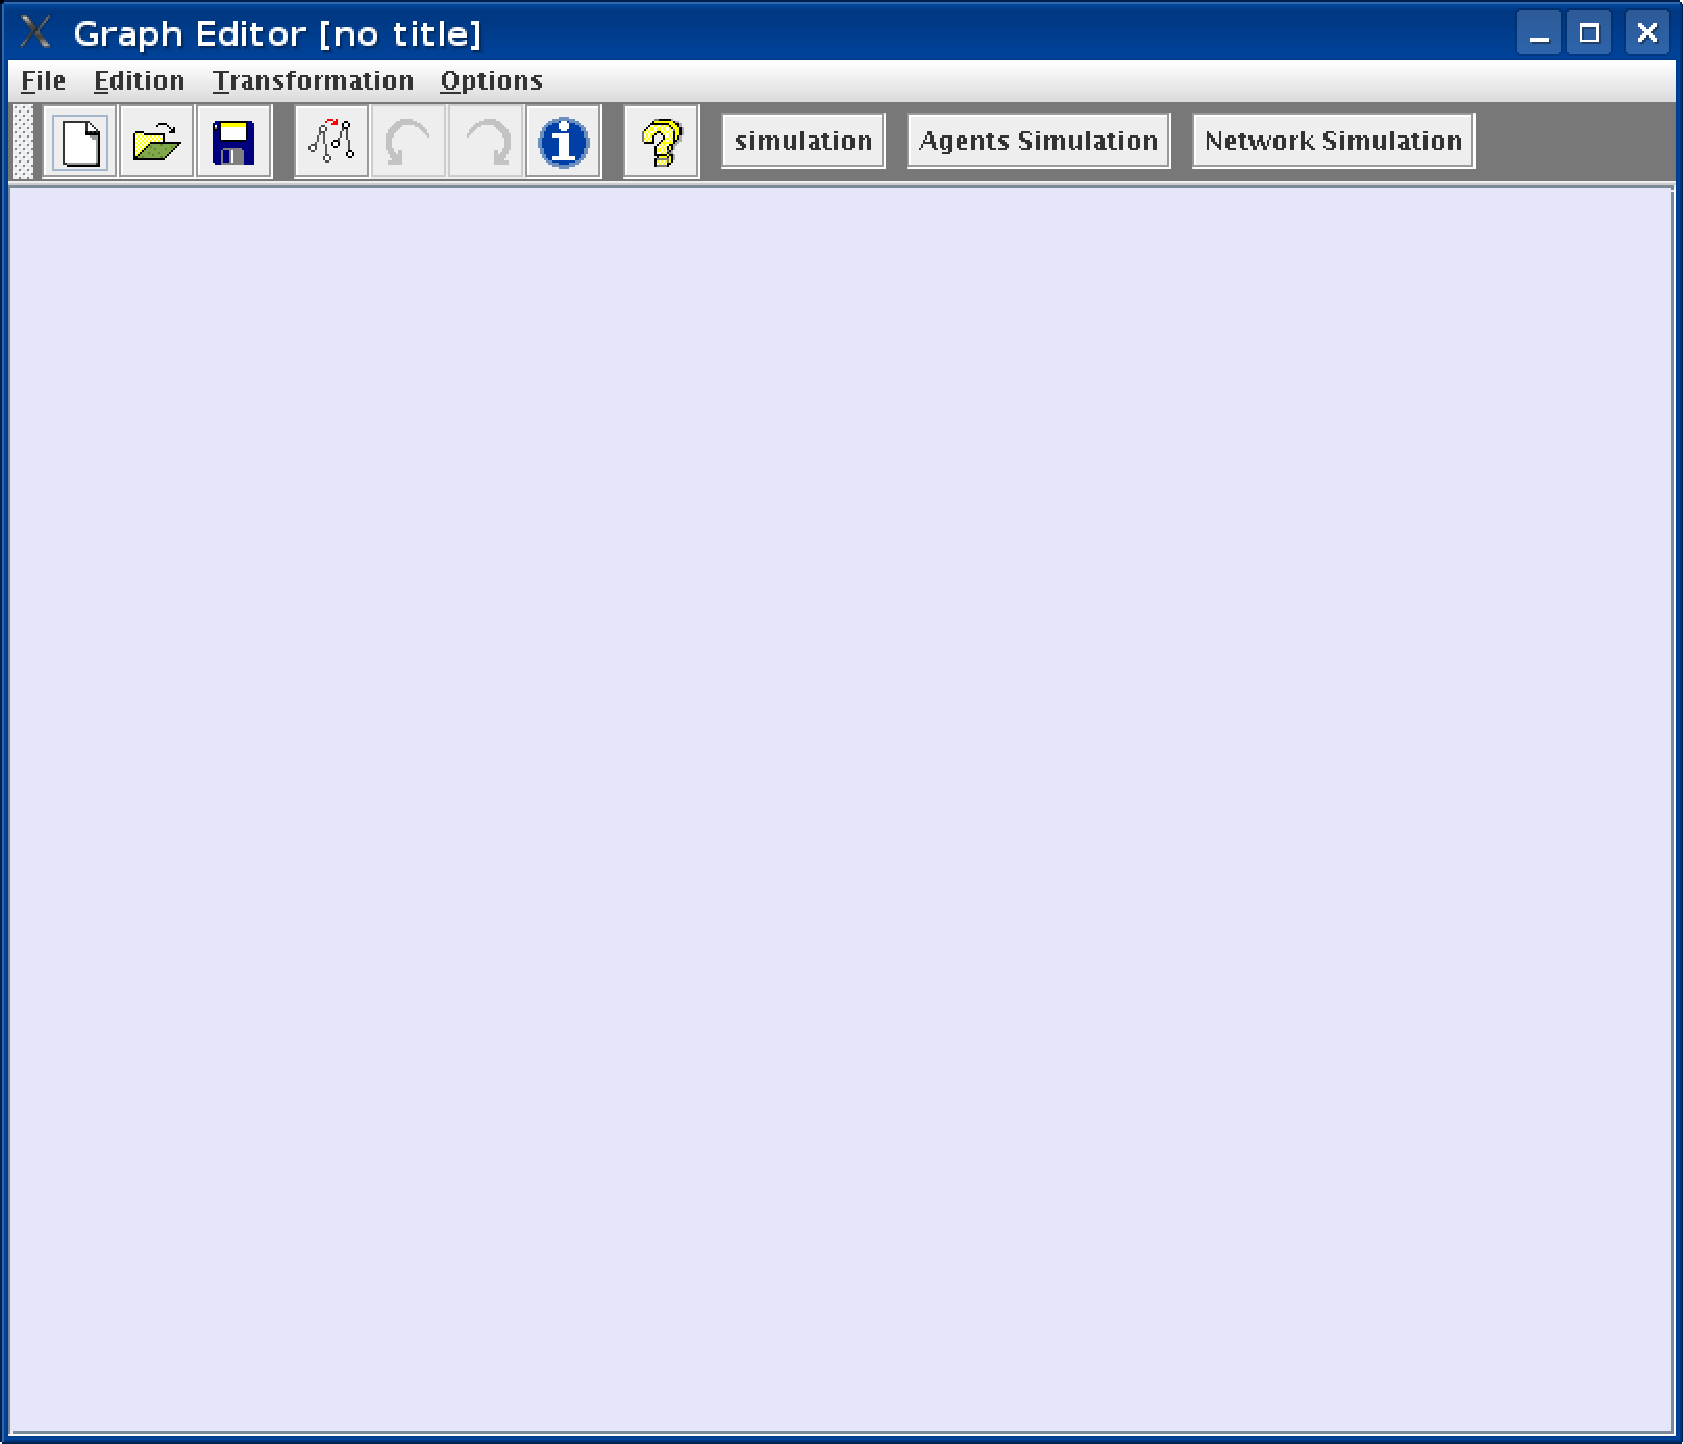
\includegraphics[width=10cm]{visidia}
  \caption{Lancement de \visidia}
  \label{fig:visidia}
\end{figure}

%%% Local Variables: 
%%% mode: latex
%%% TeX-master: "main"
%%% coding: latin-1
%%% TeX-PDF-mode: t
%%% End: 